\documentclass[14pt]{article}

\usepackage[russian]{babel}
\usepackage[utf8]{inputenc}
\usepackage{amsmath,amssymb}
\usepackage{parskip}
\usepackage{caption}
\usepackage{textcomp}
\usepackage{gensymb}
\usepackage[dvips]{graphicx}
\usepackage{wrapfig}
\usepackage{color}
\usepackage{setspace}
%\usepackage{hyperref}
\usepackage{epstopdf}

\oddsidemargin=0 cm
\evensidemargin=0 cm
\textwidth=170 mm
\textheight=230 mm
\topmargin=0 cm
\voffset= -2cm
\pagenumbering{false}
\newlength{\varheight}
\setlength{\varheight}{3.1cm}
\setlength{\parindent}{0cm}
\spacing{1.1}
\parskip=2mm
\clubpenalty=10000
\widowpenalty=10000
\captionsetup[figure]{labelformat=empty}

\begin{document}

\begin{center}
\Large{\textbf{Бесконечные цепи и сетки}}

\textbf{15.04.2017}

\vspace{5mm}
\end{center}
{\large{Цепи}}
\vspace{3mm}

1. Найдите сопротивление полубесконечной цепи (рис.)

а) при $R_1=R_2=R$,
\hspace{5cm}
б) при произвольных $R_1$ и $R_2$.

2. Определите сопротивление полубесконечной цепи между точками $A$ и $B$, если сопротивление каждого звена равно $R$ (см. рис).

3. Найдите полное сопротивление $R_{ab}$ для каждой из цепей, изображённых на рисунке.

4. Найдите сопротивление проволочной конструкции, показанной на рисунке, если сопротивление участка $AB$ равно $r_0$. Все участки сделаны из одной и той же проволоки, а количество звеньев (треугольников) в цепи очень велико. Каждый меньший равносторонний треугольник впаян в точках, делящих стороны в отношении $1:2$ (например, $AB:BC=1:2$).

5. Найдите ЭДС и внутреннее сопротивление сложного источника с бесконечным числом звеньев (см. рис). ЭДС и внутреннее сопротивление каждого отдельного элемента равны соответственно $\varepsilon$ и $r$.

6. Найдите сопротивление фрактальной цепи, изображенной на рисунке. Все звенья сделаны из одной и той же проволоки сопротивлением $\rho$ на единицу длины, сторона большого треугольника $a$, каждый следующий треугольник делит своими вершинами все стороны предыдущего пополам.

7$^*$. Рассмотрим бесконечную цепь, состоящую из катушек индуктивности и конденсаторов (см. рис). По такой цепи в отсутствие потерь могут распространяться волны. Рассмотрим случай синусоидальной волны, когда напряжение на каком-либо из конденсаторов $U(t)=U_0\cos\omega t$. При этом разность фаз между напряжениями соседних конденсаторов равна $\varphi$.

а) Выразите $\varphi$ через $\omega$ и $\omega_0=1/\sqrt{LC}$.

б) Определите линейную скорость распространения волны, если длина одной ячейки $l$.

в) При каких условиях скорость распространения волны практически не зависит от частоты $\omega$? Определите значение $v_0$ этой скорости.

\vspace{5mm}
{\large{Сетки}}
\vspace{3mm}

В задачах 8-10 считайте сопротивление ребра, соединяющего соседние узлы, известным и равным $r$.

8. Определите сопротивление при подключении между соседними узлами для разных типов сеток (см. рис):

а) квадратной,
\hspace{2cm}
б) кубической,
\hspace{2cm}
в) треугольной,
\hspace{2cm}
г) шестиугольной.

9. Определите сопротивление при подключении (см. рисунок)

а) между вершиной и серединой прилегающего к ней ребра в квадратной решетке,

б) между вершинами шестиугольной решетки ``через одну''.

10. Ученик измерил омметром сопротивление между красной и зеленой вершинами (см. рисунок) и получил значение $R_1$. Далее он измерил сопротивление между красной и желтой вершинами и получил значение $R_2$. Какое значение он получит, измерив сопротивление между красной и синей вершинами?

\begin{figure}[f]
\begin{center}
\includegraphics[width=0.48\textwidth]{infcirc1.png}
\includegraphics[width=0.48\textwidth]{infcirc2.png}
\caption{К задаче 1\hspace{7cm} К задаче 2}
\end{center}
\end{figure}
\begin{figure}[f]
\begin{center}
\includegraphics[width=0.75\textwidth]{infcirc3.png}
\hspace{0.3cm}
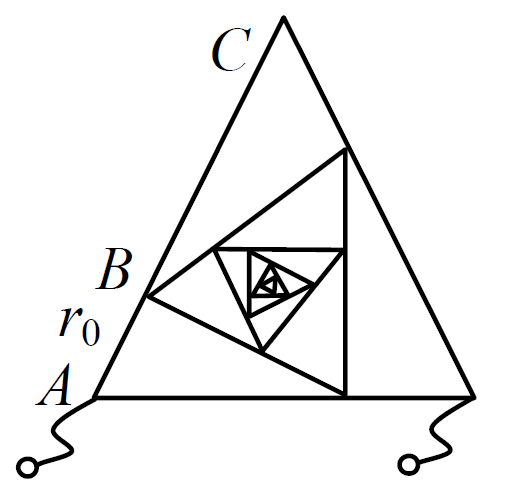
\includegraphics[width=0.2\textwidth]{infcirc9.png}
\caption{\hspace{4.7cm}К задаче 3\hspace{6.8cm}К задаче 4}
\end{center}
\end{figure}
\begin{figure}[f]
\begin{center}
\includegraphics[width=0.6\textwidth]{infcirc4.png}
\hspace{0.5cm}
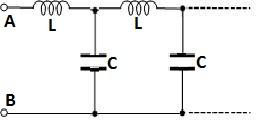
\includegraphics[width=0.33\textwidth]{infcirc5.jpg}
\caption{\hspace{2cm}К задаче 5\hspace{7cm} К задаче 7}
\end{center}
\end{figure}
%\begin{figure}[f]
%\begin{center}
%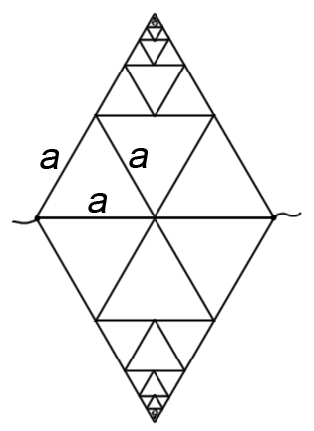
\includegraphics[width=0.28\textwidth]{infcirc8.png}
%\caption{\hspace{2cm}К задаче 6\hspace{7cm} К задаче 7}
%\end{center}
%\end{figure}
\begin{figure}[f]
\begin{center}
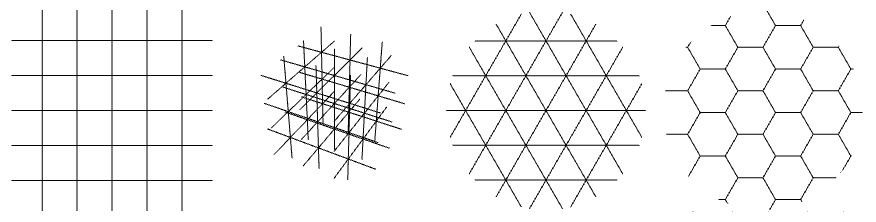
\includegraphics[width=0.99\textwidth]{infcirc6.png}
\caption{К задаче 8}
\end{center}
\end{figure}
\begin{figure}[f]
\begin{center}
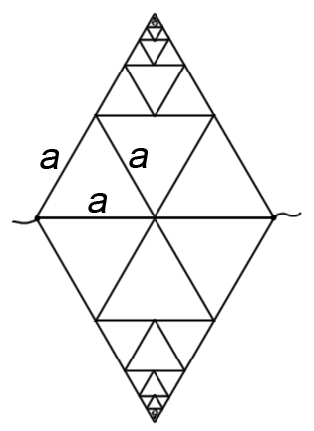
\includegraphics[width=0.18\textwidth]{infcirc8.png}
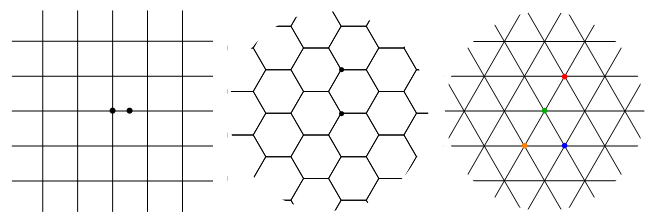
\includegraphics[width=0.75\textwidth]{infcirc7.png}
\caption{\hspace{-0.6cm}К задаче 6\hspace{2cm}К задаче 9а\hspace{2.3cm} К задаче 9б\hspace{2.3cm} К задаче 10}
\end{center}
\end{figure}

\end{document} 